\begin{frame}[allowframebreaks]{Appendix: Additional Resources}
\large
\textbf{Learning: Estimate frequencies by counting}
\normalsize
\begin{columns}
    \begin{column}{0.55\textwidth}
       \begin{itemize}
            \setlength{\itemsep}{0.75em}
            \item Recall: the goal is to estimate $p_{\text{data}}$ from samples $x^{(1)}, \ldots, x^{(n)} \sim p_{\text{data}}(x)$
            \item Suppose the samples take on values in a finite set $\{1, \ldots, k\}$
            \item The model: a histogram
            \begin{itemize}
                \item (Redundantly) described by $k$ nonnegative numbers: $p_1, \ldots, p_k$
            \end{itemize}
            \item To train this model: count frequencies
            \item $p_i = \frac{\# \text{ times } i \text{ appears in the dataset}}{\# \text{ points in the dataset}}$
        \end{itemize}
    \end{column}
    \begin{column}{0.45\textwidth}
        \begin{figure}
            \centering
            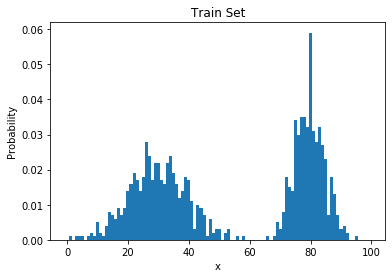
\includegraphics[width=1.1\textwidth,keepaspectratio]{images/arm/histogram_training.png}
        \end{figure}
    \end{column}
\end{columns}

\framebreak

\large
\textbf{Inference and Sampling}
\normalsize
\begin{itemize}
    \setlength{\itemsep}{0.75em}
    \item \textbf{Inference (querying $p_i$ for arbitrary $i$):} simply a lookup into the array $p_1, \ldots, p_k$
    \item \textbf{Sampling (lookup into the inverse cumulative distribution function):}
    \begin{itemize}
        \item From the model probabilities $p_1, \ldots, p_k$, compute the cumulative distribution:
        \[
            F_i = p_1 + \cdots + p_i \quad \text{for all } i \in \{1, \ldots, k\}
        \]
        \item Draw a uniform random number $u \sim [0, 1]$
        \item Return the smallest $i$ such that $u \leq F_i$
    \end{itemize}
    \item \textbf{Are we done?}
\end{itemize}

\framebreak

\large
\textbf{Problem: Lack of Generalization}
\normalsize
\begin{columns}
    \begin{column}{0.45\textwidth}
        \begin{figure}
            \centering
            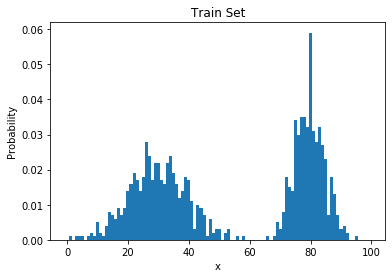
\includegraphics[width=\textwidth,keepaspectratio]{images/arm/histogram_training.png}
        \end{figure}
        \begin{figure}
            \centering
            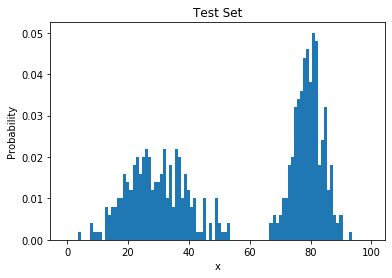
\includegraphics[width=\textwidth,keepaspectratio]{images/arm/histogram_test.png}
        \end{figure}
    \end{column}
    \begin{column}{0.55\textwidth}
       learned histogram = training data distribution 

        → often poor generalization
    \end{column}
\end{columns}

\framebreak

\large
\textbf{Solution: Parameterized Distributions}
\normalsize
\begin{columns}
    \begin{column}{0.45\textwidth}
        \begin{figure}
            \centering
            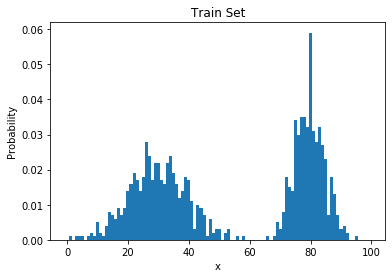
\includegraphics[width=\textwidth,keepaspectratio]{images/arm/histogram_training.png}
        \end{figure}
        \begin{figure}
            \centering
            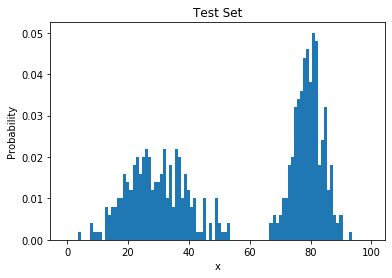
\includegraphics[width=\textwidth,keepaspectratio]{images/arm/histogram_test.png}
        \end{figure}
    \end{column}
    \begin{column}{0.55\textwidth}
       \begin{figure}
            \centering
            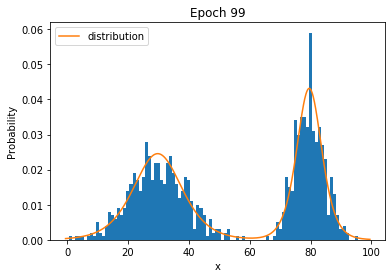
\includegraphics[width=\textwidth,keepaspectratio]{images/arm/histogram_parameterised.png}
            \caption{Fitting a parameterized distribution often generalizes better than a histogram.}
        \end{figure}
    \end{column}
\end{columns}
    
\end{frame}